
\chapter{Basics}
\label{ch:basics}

% This section should explain the basic math to understand the aforementioned topics, not that much needed but still needs to be there.

\section{Sampled Data, Grids and (Uncertain) Fields}
\label{sec:uncertainfields}

The goal of this section is to give insights into the structure of scientific (sampled) data, grids, interpolation, and (uncertain) fields. 
Especially the first parts of this section are largely based on the work of \citeauthorwork{telea2014data}, for a more extensive introduction please refer to it. 

\subsection{Sampled Data, Grids and Interpolation}

In general, data can be classified into two categories: intrinsically continuous or intrinsically discrete data. 
The latter refers to data such as websites, texts, source code, images or any other type of record. 
The first on the other hand usually stems from nature and is measured in physical units like $kg$, $\frac{m}{s}$ or similar.
Continuous data conforms to the Cauchy-Criterion (also called the $\epsilon - \delta$-Criterion), which essentially states that a function $f(x)$ is uniformly continuous if, for any small amount $\epsilon$ you choose, you can find a small distance $\delta$ such that whenever two points are within $\delta$ of each other, their function values are within $\epsilon$ of each other (see \cite{telea2014data} for the mathematical definition). 
Continuous data can be mathematically represented as a function in the form of \cite{telea2014data}:

\begin{equation}
  f: D \rightarrow C
  \label{eq:continous data}
\end{equation}

With $D \subset \mathbb{R}^d$ and $C \subset \mathbb{R}^c$. 
In this case the function is called a d-dimensional, c-valued function, which means it maps from its original function domain $D$ to values in the $C$ domain. 
Functions with $c=1$ are called Scalar Fields, assigning every position in the function domain a single scalar attribute $x \in \mathbb{R}$. 
Vector Fields ($c=2$ or $c=3$) on the other hand assign every position a vector in the form of $(x_1, x_2) \in \mathbb{R}^2$ or $(x_1, x_2, x_3) \in \mathbb{R}^3$, which can (but does not have to) depend on the original function domain. 
There are also fields related to higher dimensions (Tensor fields), but they are beyond the scope of this Thesis. 

Although this kind of data is continuous in the real world, its computational representation is nearly always discrete. 
The reason for this is that it is a) hard to achieve continuous data and b) many mathematical operations (e.g. filtering, denoising, rendering) are hard to perform on continuous data. 
According to \citeauthorwork{telea2014data}, this is called \textit{sampled data} and could come from e.g. measurements or computer simulations. 
The sampled data can then be used to reconstruct the original, continuous dataset by using interpolation. 
Therefor, when a field is mentioned in this Thesis, it usually refers to such an approximation of a continuous field like in Equation~\ref{eq:continous data}. 


Interpolation usually uses the structure of data, which is mostly called a \textit{grid} (or sometimes mesh). 
A grid is a subdivision of the original function domain $D$ into a non\--overlapping collection of cells, which in turn are spanned by vertices, which are the sample points of the discretization of the continuous field.  
There are multiple ways of defining grids (e.g. rectilinear, structured, unstructured, see Figure~\ref{fig:grid types}) and cells (examples for 2D: line, triangle, quad, hexahedron), but for the sake of brevity this section only introduces the grid applied by the dataset used for this Thesis: The uniform grid. 

\begin{figure}
  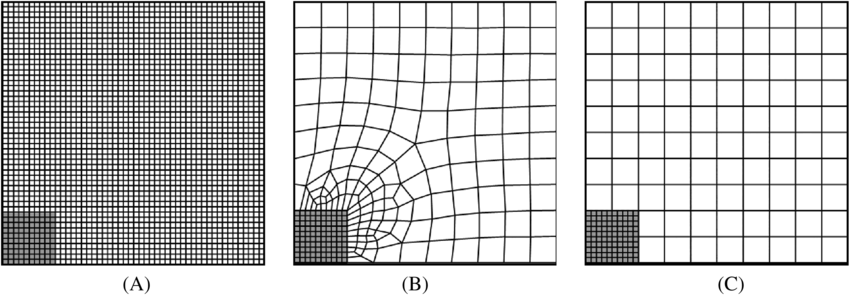
\includegraphics[width=0.95\textwidth]{figures/grid-types.png}
  \caption{Different types of Grids: A) Uniform Grid, B) unstructured grid, and C) no-conforming grid from \cite{kaltenbacher_nonconforming_2022}}
  \label{fig:grid types}
\end{figure}


A uniform grid is essentially an axis-aligned box spanning over the original function domain $D$. 
The extent of the box can be described as a list of $d$ pairs:

\begin{equation}
  ((m_1, M_1),\dots,(m_d, M_d)), (m_i, M_i) \in \mathbb{R}^2, m_i < M_i
  \label{eq:uniform grid coordinates}
\end{equation}

$(m_i, M_i)$  make up the lower and upper limit of the extent in each axis' direction. 
The sample points are then uniformly distributed along the axis with a given distance $\delta_i$ depending on the axis and all sample points $p_i$ can be described with: 

\begin{equation}
  p_i = (m_1 + n_i\delta_i,\dots, m_d + n_d\delta_d), n_1, \dots, n_d \in \mathbb{N}
  \label{eq:smaple point uniform grid}
\end{equation}

Therefor, every sample point can be described by its integer coordinates $n_1, \dots, n_d$. 
The number of sample points on axis $i$ is then $N_i = 1 + (M_i - m_i)/\delta_i$, and the set $(N_1, \dots, N_d)$ is often called the \textit{shape} of the uniform grid.   
The benefits of using uniform grids are the very low storage requirements ($3d$ floating point numbers, regardless of its size) and its simple implementation. 
Drawbacks are mainly that uniform grids do not represent all use-cases well or require an unnecessary high density to do so. 


Interpolation is the process of reconstructing the continuous data $f$ (Equation~\ref{eq:continous data}) from sampled points $p_i$ and associated values $f_i$. 
In general, there are multiple ways of interpolating, for example using by using \textit{nearest-neighbor interpolation}, assigning each point the value of the closest cell center. 
While this is computationally efficient, it is a staircase-like, discontinuous approximation of the original data. 
A better, continuous approach is linear interpolation, which interpolates the value of a point $x \in D$ based on the surrounding cell. 
But since interpolation is handled at the very last, visualization step (and handled by libraries), the full mathematical description (and other interpolation ideas) are out of the scope of this Thesis, but are detailed in \citeauthorwork{telea2014data}. 

\subsection{Map Projections}

Regarding the original function dimension $d$ of the field $f$ described in Equation~\ref{eq:continous data}, there is a subtle but important distinction: the \textit{geometrical dimension} versus the \textit{topological dimension}. 
The geometrical dimension refers to the dimension of space $D$ is embedded in ($d$), while the topological dimension refers to the actual function domain $D$ itself, which is $s\leq d$ \cite{telea2014data}.
The difference is best illustrated with the example of the application in this Thesis: simulating earth's surface. 
Since the earth is a three-dimensional object, and also the earths surface is (approximately) a sphere's surface, the geometrical dimension of such datasets is $d=3$. 
But since the earths surface can be is a (curved) plane, the topological dimension of such datasets is $s=2$, which is also the reason why it is enough to access any gridpoint on earths with two coordinates: \textit{latitude} (lat), referring to the degrees on the north-south axis, and \textit{longitude} (lon), referring to degrees on the east-west axis.
Typically, since the topological dimension is the more relevant one, it is referred to as the \textit{dataset dimension}, while the geometrical dimension is mostly assumed to be three. 

\begin{figure}[htp]
  \begin{center}
    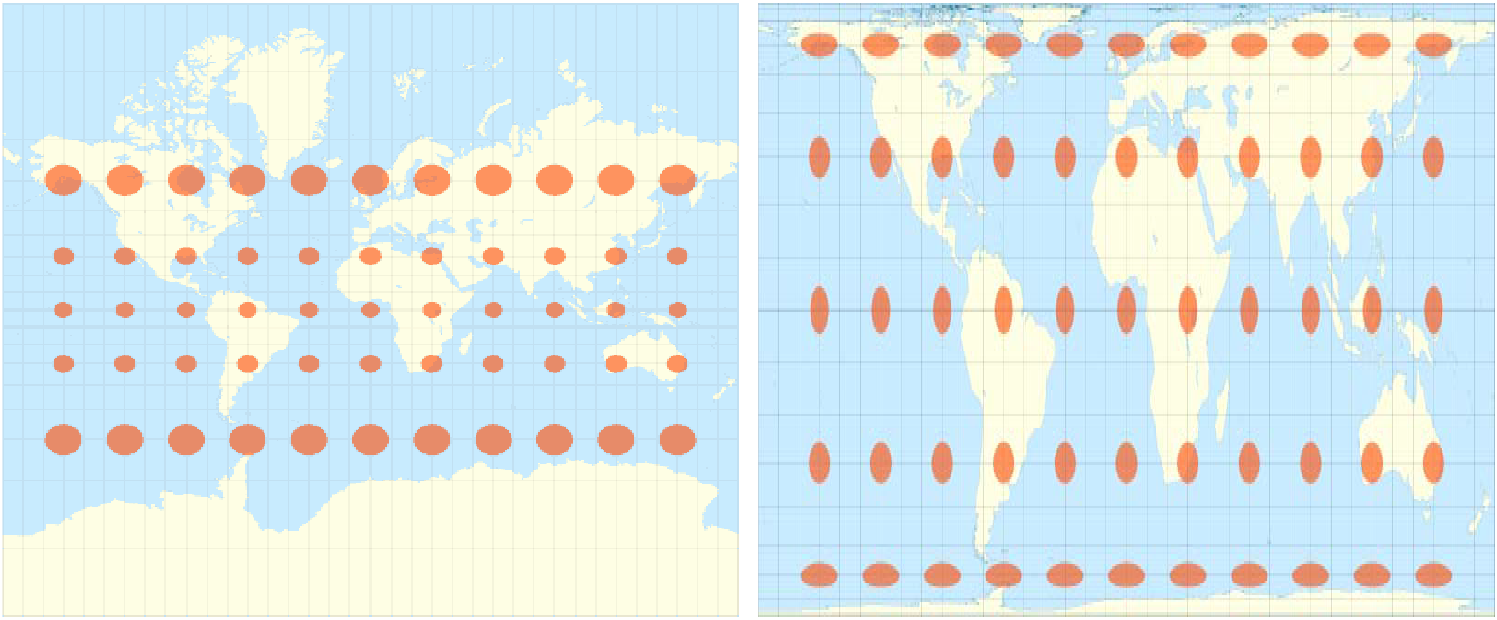
\includegraphics[width=0.95\textwidth]{figures/tissot-map-projections.png}
  \end{center}
  \caption{Two different map projections with different kinds of warping, depending on the map projection. The amount of warping is indicated by Tissot’s indicatrices (orange circles). Left: Mercator Projection, Right: Lambert Equal-Area Projection \cite{ghaderpour_map_2014}}\label{fig:tissot map projections}
\end{figure}


Unfortunately, this requires the mapping of a 2D paper plane to a 2D sphere surface, which is topologically impossible (without distortions) \cite{vietinghoffdiss}.
Therefor, numerous different map projections were invented, which all have a different kind of distortion in different geographical places. 
Figure~\ref{fig:tissot map projections} shows two distinct projections, both with their own advantages and disadvantages. 
As pointed out by \citeauthorwork{vietinghoffdiss}, a different map projections may fit the area of interest better, the Mercator projection in Figure~\ref{fig:tissot map projections} (left) is still chosen for this thesis, due to limitations in the employed map projections library (see Section~\ref{sec:vis_analysis}). 
This distortion also plays a role in calculations with uniform lon/lat-grids, since coordinates in the far north (and south) are vastly overrepresented, since they actually refer to a far smaller portion of the earth's surface than data near the equator (see Section~\ref{sec:eof} for geographical weighting). 


\subsection{Uncertain Fields}

% Explain uncertain fields and ensembles from \cite{vietinghoffdiss, pothkow2015modeling}

As already mentioned, the results of GCMs are often multiple simulations. 
Mathematically, this is defined as an \textit{uncertain} or \textit{random field}. 
Since all fields used in this Thesis are scalar fields, we will define uncertain fields only for those. 
Let's assume $s : D \rightarrow \mathbb{R}$ is a scalar field, associating a value  with every point in $D$. 
As mentioned in the previous section, such fields are usually approximated using $n$ sample points in a grid $(x_1,\dots, x_n) \in D^n$ and their associated scalar values, represented in a vector $(s_1,\dots,s_n) \in \mathbb{R}^n$ ($s_i$ is the scalar value at grid point $x_i$).
This being a \enquote{normal} (or rather deterministic) scalar field, an uncertain scalar has no concrete given values $s_i$ but follows an unknown probability density \cite{vietinghoffdiss}, which is illustrated in Figure~\ref{fig:uncertain field example}. 


\begin{figure}[htb]
  \begin{center}
    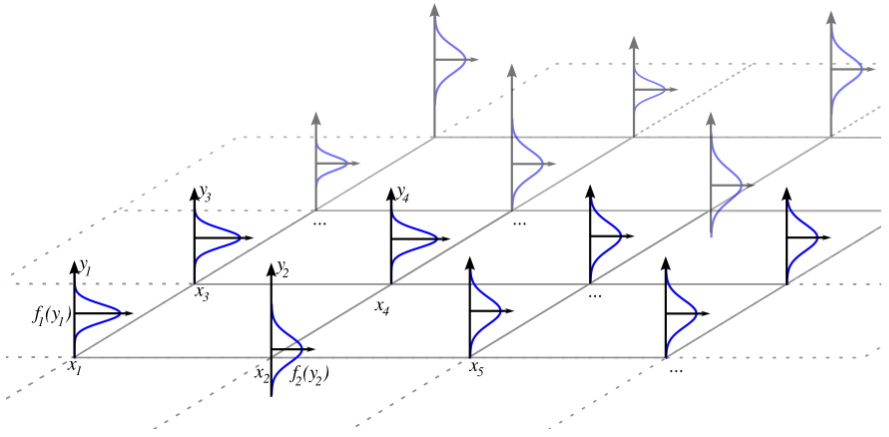
\includegraphics[width=0.95\textwidth]{figures/uncertain_gaussian_field.png}
  \end{center}
  \caption{Illustration of an uncertain field with a Gaussian probability density function at every sample point (from \cite{pothkow2015modeling})}
  \label{fig:uncertain field example}
\end{figure}

For similar reasons why continuous data is available mostly in discrete form, the probability density function (PDF) associated with every sample point is in practice rarely given as the actual function, but rather as sampled values. 
In the case of this Thesis, these samples stem from multiple \textit{realizations} $\omega \in \Omega$ ($\Omega$ being the sample space, which represents the different samples of the PDF), wich associates every realization with one version of the field: $F: \Omega \rightarrow \mathbb{R}^n$.
With regard to simulations, one realization $\omega$ is associated with a certain set of parameters for a mathematical model. 
Again, the full set of $\Omega$ cannot be realized, so a certain number $m$ of realizations $Z = (\omega_1,\dots,\omega_m) \in \Omega^m$ is used to approximate the PDFs associated with each grid point. 
Connecting this with the terms mentioned in Section~\ref{sec:climate research}: The set of fields $F(Z)$ is called \textit{ensemble}, while each field $F(\omega_i), i \in {1,\dots,m}$ is the $i$th \textit{member} (or \textit{realization}) of said ensemble. \cite{vietinghoffdiss}  
% With $x_i \in \D, i \in {1, 2, \dots, M}$ (the approximation of $D$ in Equation~\ref{eq:continous data}), 


\section{Empirical Orthogonal Functions}
\label{sec:eof}


\subsection{Overview}

Empirical Orthogonal Functions (short: EOFs) analysis, also known as geographically weighted PCA or Proper Orthogonal Decomposition \cite{vietinghoffdiss}, \enquote{is among the most widely and extensively used methods in atmospheric science} \cite{hannachi_empirical_2007}. 
One of its goals is to reduce the usually very high dimensionality of atmospheric data and can be used to link certain modes/patterns to the physics/dynamics of the analyzed system.  
EOFs are a statistical procedure to decompose spatio-temporal data into two components: On the one hand orthogonal spatial patterns, on the other hand corresponding uncorrelated temporal coefficients, representing the activity of their corresponding pattern in certain time steps \cite{hannachi_empirical_2007, vietinghoffdiss}. 
The naming of the components is for from being consistent: The spatial patterns are also called spatial modes, PC loadings, EOFs or even sometimes PCs, while the temporal coefficients are also named principal components (PCs), EOF amplitudes or EOF (expansion) coefficients \cite{hannachi_empirical_2007}. 
So as a formula, a spatio-temporal field $X(t, s)$ (e.g. a sea level pressure field over time mentioned in Section~\ref{sec:nao}) can be described as

\begin{equation}
  X(t, s) = \sum^{M}_{k=1} c_k(t) u_k(s)
  \label{eq:eof decomposition}
\end{equation}

with $M$ being the number of modes/patterns and  $c_k$ the $k$th temporal coefficients and $u_k$ the spatial pattern \cite{hannachi_empirical_2007}. 

This could be achieved with multiple kinds of decomposition, but EOF tries finding new sets of variables ($c_k(t)$ and $u_k(s)$ from Equation~\ref{eq:eof decomposition}) that each capture a maximum possible amount of variance/variability of the original dataset. 
So the first of $M$ modes captures the most variance, the second one the second most and so on. 

\subsection{Mathematical Derivation and Computation of EOFs}

The goal of this Section is to give an overview of the mathematical origins of EOFs based on the work of \citeauthorwork{hannachi_empirical_2007} as well as their actual practical computation. 
For a more in depth history and derivation, please refer to \cite{hannachi_empirical_2007} and their references, while \citeauthorwork{weiss_tutorial_2019} gives a great hands-on tutorial on POD/EOFs and their interpretation and computation. 

As already explained, the starting point of EOFs is usually a spatio-temporal field $X(t, s)$ defined on a Grid $G$ over $n$ time steps, for example the precipitation analyzed in this Thesis. 
The value at each grid point at geographical location $s_j$ and time $t_i$ is given as $x_{ij}$, with $i = 1, ..., n$  and $j = 1, ..., p$.  
The first step is usually to remove the climatology of the dataset to turn it into anomaly maps. 
The climatology is usually defined as the temporal mean $\bar{x}$ of the analyzed datachunk, so 
\begin{align}
  \bar{x}_i = \frac{1}{n} \sum^{n}_{k=1} x_{ki} \\
  \bar{x} = (\bar{x}_1, ..., \bar{x}_p)^T .
  \label{eq:climatology}
\end{align}

So the values of anomaly maps $x'_{ij}$ at each grid point are given as the departure of $X$ from its climatology: 



\begin{equation}
  x'_{ij} = x_{ij} - \bar{x}_j \\
  \label{eq:anomaly map elements}
\end{equation}

And so the final anomaly map $X'$ is: 
\begin{equation}
  X' = \begin{pmatrix}
x'_{11} & x'_{12} & \cdots & x'_{1j} \\
x'_{21} & x'_{22} & \cdots & x'_{2j} \\
\vdots & \vdots & \ddots & \vdots \\
x'_{i1} & x'_{i2} & \cdots & x'_{ij}
\end{pmatrix}
  \label{eq:anomaly map}
\end{equation}

% Since from here on only anomaly maps are considered in the derivation and calculation of EOFs, the $'$ gets omitted and $X$ stands now for the anomaly data.  
The first usual step for generating EOFs is the covariance matrix defined by 

\begin{equation}
  S = \frac{1}{n} X'^T X' 
  \label{eq:covariance map}
\end{equation}

This covariance matrix with the values $s_{ab}$ with $a,b = 1, \cdots, p$ contains the covariance of any grid point with any other grid point over the time. 
To find EOFs means determining a unit length direction $u = (u_1, \cdots, u_p)$ that explains the most variability. 
This problem is therefor equivalent to the solution to the eigenvalue problem, so finding all the eigenvectors ($\equiv$ EOFs) and their eigenvalue. Which means that the vector $u$ multiplied by the covariance matrix $S$ is equivalent to the multiplication with a scalar $\lambda^2$ (the eigenvalue):  

\begin{equation}
  Su = \lambda^2 u
  \label{eq:eigenvalue problem} 
\end{equation}

So to find the $k$th EOF of a Covariance matrix, the eigenvectors $u$ are sorted by the (largest first) value of their corresponding eigenvalue $\lambda^2$. 
The primary (or dominant) EOF the first in this order, the secondary EOF the second and so on. 
The variance $v_k$ of the original dataset associated with the $k$th EOF can then be calculated with: 

\begin{equation}
  v_k = \frac{\lambda^2_k}{\sum^{p}_{i=1} \lambda^2_i}
  \label{eq:eof variance calculation}
\end{equation}

The temporal coefficients can then in turn be calculated projecting the eigenvectors $u_k$ on the original anomaly map $X'$ with: 

\begin{equation}
  a_{k} = X'u_k
\end{equation}

Together they fulfill the requirements of the decomposition in Equation~\ref{eq:eof decomposition}. 
% So the coefficients in Equation~\ref{eq:eof decomposition}
Note here that the solutions being eigenvectors means that the multiplication by any scalar $\alpha$ (i.e. $\alpha u_k$ and $\alpha^{-1} a_k$) is also a valid solution to the problem. 
This leaves room of choosing scale and direction in a useful way (see Section~\ref{sec:eof_calc} for a practical implementation) \cite{vietinghoffdiss}. 

\subsection{Calculation and Application to the geographical Domain}


Since geographical data is usually given on a regular 2D grid which depicts the earth's surface, the influence of grid point density (same degree resolution is far more sparse in equatorial regions than in the Arctic) need to be corrected with geographical weights. 
Those can be approximated by the square root of the cosine of the respective latitude \cite{hannachi_primer_nodate, vietinghoffdiss} with a similar diagonal matrix as depicted in \cite{hannachi_primer_nodate}: 

\begin{equation}
  W = \begin{pmatrix}
    \cos(\theta_1) & 0 & \cdots & 0 \\
0 & \cos(\theta_2) & \cdots & 0 \\
\vdots & \vdots & \ddots & \vdots \\
0 & 0 & \cdots & \cos(\theta_p)
\end{pmatrix}
  \label{eq:geographical weighting}
\end{equation}
  

Fortunately, there is no need to calculate the covariance matrix and solve the eigenvalue problem. 
Linear Algebra provides a tool called \textit{Singular Value Decomposition} (SVD), which decomposes any matrix $X$ into three components: 

\begin{equation}
  X = L \Lambda R^T 
  \label{eq:svd definition}
\end{equation}

$L$ contains the left singular vectors, $R$ the right singular vectors and $\Lambda$ a diagonal matrix containing the singular values $\lambda_k$ (as used in Equation~\ref{eq:eof variance calculation} above). 

Now all of the above is used to calculate the EOFs of geographical data by applying SVD to the matrix (like in \citeauthorwork{vietinghoffdiss}): 

\begin{equation}
  \tilde{X} = \frac{1}{\sqrt{n - 1}} W^{\frac{1}{2}} X' 
  \label{eq:complete data preperation}
\end{equation}


When using SVD of $\tilde{X}$ with time as the first dimension (like depicted here), the columns of $R^T$ are the EOFs (so $u_k(s)$ of Equation~\ref{eq:eof decomposition}) and the columns of $L$ multiplied with $\sqrt{n - 1}$ are the principal components or EOF coefficients ($c_k(t)$ in Equation~\ref{eq:eof decomposition}).
As explained above, this result can be scaled, which is explained in detail in Section~\ref{sec:eof_calc}.
\todo{go over this whole section and check everything for being correct!!!!}



